\documentclass[11pt, letterpaper]{article}
\usepackage[utf8]{inputenc}
\usepackage[english]{babel}
\usepackage[in]{fullpage}
\usepackage[pdftex]{graphicx}
\graphicspath{{./img/}{./graphs/qos/}{./graphs/adm/}}
\usepackage{subfig}
\usepackage{amssymb}
\usepackage{setspace}
\usepackage{multirow}
\usepackage{rotating}
\usepackage[hidelinks]{hyperref}
\usepackage{url}
\usepackage{xcolor}
\usepackage{colortbl}
\usepackage{acronym}
\usepackage[square,numbers]{natbib}
\usepackage{logo-ic}
\usepackage{booktabs}

\definecolor{lightgray}{gray}{0.75}

\usepackage{csquotes}


\newcommand{\TODO}[1]{{\color{red} #1}}
\newcommand{\x}{$\bullet$}
\newcommand{\m}{$\checkmark$}

% Hyperref configuration
\hypersetup {
  pdftitle={Doctoral Qualifying Exam -- Luciano Jerez Chaves},
  pdfauthor={Luciano Jerez Chaves},
  pdfcreator={pdfTeX 3.14159265-2.6-1.40.16 (TeX Live 2015)},
  pdfsubject={Doctoral Qualifying Exam - IC/UNICAMP},
  pdfkeywords={Software-Defined Networking, OpenFlow protocol, Long Term
  Evolution, Network Management},
}

\begin{document}

\def\sectionautorefname{Section}
\def\subsectionautorefname{Section}
\def\subsubsectionautorefname{Section}
\def\figureautorefname{Figure}
\def\subfigureautorefname{Figure}
\def\tableautorefname{Table}

\sloppy

\pagenumbering{roman}
\thispagestyle{empty}

% Logos and names
\begin{center}
  \begin{tabular}{ccc}
    \raisebox{-.5\height}{
\includegraphics[width=2.2cm]{logo-unicamp}}
    &
    \begin{minipage}{.6\textwidth}
      \centering
      \textbf{Universidade Estadual de Campinas} \\
      \textbf{Instituto de Computação} \\
    \end{minipage}
    &
    \raisebox{-.5\height}{\scalebox{1.11}{\LogoIcUnicampWithName}}
  \end{tabular}
\end{center}
  
\hrule
\vspace{2cm}

\begin{center}
  {\large \textbf{Exame de Qualificação de Doutorado}} \\
  \vspace{1.5cm}
  {\Large \textbf{Future Generation Multi-tier Video Delivery for Smart Cities}} \\
  \vspace{1.5cm}
      \begin{tabular}{rl}
          \textbf{Candidate}:  & Eduardo de Souza Gama \\
          \textbf{Orientador}:    & Luiz Fernando Bittencourt, D.Sc. \\
          \textbf{Co-orientador}: & Roger Immich, D.Sc. \\
      \end{tabular}
  \vspace{0.25cm}

  \begin{abstract}%
  \onehalfspacing

  The world is witnessing a rapid growth in mobile communication, and network
  operators have been forced to handle network traffic more resourcefully. Many
  works point to the use of \ac{SDN} as an enabling technology to overcome
  current limitations, making possible upcoming 5G networks. This doctoral
  research project discusses how the \ac{SDN} paradigm and the OpenFlow
  protocol can be integrated into existing \ac{LTE} networks, going through the
  state-of-the-art solutions and highlighting some open issues in the area.
  Some contributions have already been developed, as the new OpenFlow module
  for \ac{SDN}-based \ac{LTE} networks simulations, and a complete \ac{LTE}
  \acs{QoS} realization with OpenFlow protocol. Taking into account that future
  5G heterogeneous networks will become much denser with many more cells,
  contributions are proposed toward a scalable controller architecture,
  including a distributed mobility management and algorithms for traffic
  offloading between different cells, and even between different technologies.
  Through solutions developed in this research, it is intended to enable more
  agile and flexible mobile networks, lowering management costs for network
  operators and improving the experience for users.

  \end{abstract}
  \vspace{0.5cm}
  Dezembro, 2019 %\today
\end{center}
\newpage
\mbox{}

\newpage
\tableofcontents
\newpage
\mbox{}

\newpage
\section*{Lista de Acrônimos}

\vspace{0.8cm}

\begin{acronym}[CSMA/CA]
	\itemsep0.5pt
	\acro{QoE}      {Quality of Experience}
	\acro{HTTP}     {HyperText Transfer Protocol}
	\acro{HAS}		{HTTP Adaptive Streaming}  
	\acro{DASH}		{Dynamic Adaptive Streaming over HTTP}  
	\acro{NIST}		{National Institute of Standard and Technology}
	\acro{ISP}		{Internet Service Provider} 
	\acro{BBU}		{Baseband Unit}
	\acro{HTML5}	{HyperText Markup Language, version 5} 
	\acro{ABR}		{Adaptation BitRate}
	\acro{SDN}      {Software Defined Networking}
	\acro{NFV}      {Network Function Virtualization}
	\acro{ns-3}     {Network Simulator~3}
	\acro{CDN}      {Content Delivery Network}
	\acro{CACA}     {Content-aware Cache Admission}
	\acro{NDN}      {Named Data Network}
	\acro{LTE}      {Long Term Evolution}
	\acro{PoP}      {Point of Presence}
	\acro{RDMA}     {Remote Direct Memory Access}
	\acro{MCFP}     {Multi-Commodities Flow Problem}
	\acro{GTA}      {Game Theory Algorithm}
	\acro{MLP}      {Multilayer Perceptron}
	\acro{ILP}      {Integer Linear Programing}
	\acro{VoD}      {Video on Demand}
	\acro{ILP}      {Integer Linear Programing}
	
\end{acronym}



\newpage
\pagenumbering{arabic}
\setcounter{page}{1}
\onehalfspacing

\section{Introduction}
\label{ch:introduction}

%******* Introduction of the Dash technology and Cloud/Fog networks****


% ----------------------------------------------------------------------------
% What is the current context in mobile network in terms of traffic and users? 
% ----------------------------------------------------------------------------
Os serviços de streaming de vídeo representam a maior parte do tráfego da Internet. De acordo com as previsões da Cisco~\footnote{Visual Networking Index: atualização global de previsão de tráfego de dados móveis. Link:~\url{http://shorturl.at/hjAZ1}. Acesso em: 29 de julho de 2019.}, em 2021, 70\% de todo o tráfego da Internet será dominado por streaming de vídeo. Isso inclui os serviços de vídeo atuais, bem como serviços inovadores de jogos na nuvem e futuros consoles~(por exemplo, Google Stadia), enquanto que para dispositivos móveis, essa estimativa representa 78\% de todo o tráfego de dados. Essa tendência impõe novos desafios no fornecimento de vídeos com a melhor \acl{QoE}~(QoE), originalmente projetada considerando o modelo de \textit{best-effort} para transmissão de dados.

% ----------------------------------------------------------------------------
% What carries have been doing to address the increasing traffic?
% ----------------------------------------------------------------------------
% Em cenários para as futuras gerações da Internet, tecnologias de redes sem fio, como, redes 5G, mobile-edge computing~(MEC), redes definida por software~(SDN).
%Esses fatores demonstram como o futuro da demanda da Internet pode se tornar muito grande para os ISPs e os avanços tecnológicos nas telecomunicações nas quais eles dependem. 
Atualmente, os tradicionais serviços de Streaming de vídeo são projetados para distribuir conteúdo multimídia atraves de grandes data centers na nuvem. Esses sistemas na nuvem geralmente usam um conjunto de servidores em que o tráfego passa pelo núcleo da rede; além disso, de modo geral, a conexão dos dispositivos é feita por usuários estáticos e por links de Internet estáveis [?]. Dessa forma, a criação desses sistemas resolve parcialmente os problemas de escalabilidade, disponibilidade e interoperabilidade, mas ao mesmo tempo, apresenta novos desafios (por exemplo, maior latência e congestionamento da rede principal) [?]. Vários trabalhos na literatura destacam a computação de nevoa/borda para lidar com as novas demandas de tráfego de video que estão surgindo. Onde datacenters com menos capacidade de processamento e armazenamento conseguem prover serviços/virtualização mais próximos ao usuário final. Assim, a borda da rede pode fornecer taxas de latência que a nuvem não conseguem alcançar de outra forma [?], [?].
% ou caches especificos alocados pelo proprio administrador da rede

%, levando em consideração as novas tecnologias que estão surgindo, como, redes 5G, mobile-edge computing~(MEC), redes definida por software~(SDN)

% A Fig. 1 Mostra ao longo de cada ano o crescimento no consumo de banda, estes tipos de cenários impõem significantes desafios para a distribuição de vídeo sobre as futuras gerações da Internet.
Pra acomadar a demanda de streaming de video, crescendo exponencialmente, bem como manter o QoE do usuário, grandes players como Microsoft, Apple, Adobe e Netflix adotam o paradigma de streaming adaptável sobre HTTP~(HAS). Como a maioria das soluções HAS usa a mesma arquitetura, o Motion Picture Expert Group~(MPEG) propôs um padrão chamado Dynamic Adaptive Streaming over HTTP~(DASH), no qual o player de vídeo do cliente pode escolher dinamicamente o nível de taxa de bits de acordo com a largura de banda disponível percebida..
%Atualmente, esses conteudos multimidia utilizam serviços de Streaming Adaptativo Dinâmico sobre HTTP~(HAS), este paradigma trata o video multimídia como qualquer outro conteúdo comum da Web e o entrega em pequenos pedaços atraves do protocolo HTTP.
%Os serviços de transmissão de vídeo têem seu bitrate adaptados dinâmicamente.% As soluções HAS utilizam os protocolos HTTP na aplicação e TCP na camada de transporte como ilustrados na figura 1b. 
%em Streaming Adaptativo Dinâmico sobre HTTP~(DASH) são amplamente adotado por provedores de vídeo como Google, Netflix, Akamai HD e outros, nos quais o player de vídeo do cliente pode escolher dinamicamente o nível de taxa de bits de acordo com a largura de banda disponível percebida.
Esta solução emprega adaptação dinâmica em relação às condições de rede variáveis para fornecer uma experiência de streaming contínua~(ou pelo menos mais suave). Depois que um arquivo de mídia~(ou fluxo) estiver pronto a partir de uma fonte, ele será preparado para transmissão em fluxo antes de ser publicado em um servidor HTTP padrão e pronto para uso.

%HAS uses HTTP as the application and TCP as the transport-layer protocol as illustrated in Figures 1.2b and 1.3, and clients pull the data from an HTTP server. HAS solutions employ dynamic adaptation with respect to varying network conditions to provide a seamless (or at least smoother) streaming experience. Once a media file (or stream)is ready from a source, it is prepared for streaming before it is published to a standard, off-the-shelf HTTP server. The original file/stream is partitioned into segments (also calledchunks) of equi-length playback time, and multiple versions (also called representations)of each segment are generated that vary in bitrate/resolution/quality using an encoder ora transcoder (i.e., H.264, H.265, etc.). Moreover, the server generates an index file, whichis a manifest that lists the available representations including HTTP uniform resourcelocators (URLs) to identify the segments along with their availability times. During atypical HAS session, the client first receives the manifest that contains the metadata forthe video, audio, subtitles, etc., and then constantly measures certain parameters such as the available network bandwidth, buffer status, and battery and CPU levels. According tothese parameters, the HAS client repeatedly fetches the most suitable next segment amongthe available representations from the server. Table 1.1 compares the main characteristicsof the traditional streaming and HAS systems.

% ----------------------------------------------------------------------------
% What carries have been doing to address the increasing traffic?
% ----------------------------------------------------------------------------
%Em cenários para as futuras gerações da Internet, tecnologias de redes sem fio, como, redes 5G, mobile-edge computing~(MEC), redes definida por software~(SDN).
%Esses fatores demonstram como o futuro da demanda da Internet pode se tornar muito grande para os ISPs e os avanços tecnológicos nas telecomunicações nas quais eles dependem. 
%Atualmente, tradicionais serviços de Streaming de vídeo sob Demanda~(VoD) são projetados para distribuir conteúdo multimídia por grandes data centers na nuvem. Esses sistemas geralmente usam um conjunto de servidores em que o tráfego passa pel núcleo da rede; além disso, a conexão dos dispositivos é feita por usuários estáticos e por links da Internet estáveis [?]. Dessa forma, a criação desses sistemas no nível da nuvem resolve parcialmente os problemas de escalabilidade, disponibilidade e interoperabilidade, mas ao mesmo tempo, apresenta novos desafios (por exemplo, maior latência e congestionamento da rede principal) [?]. Vários trabalhos na literatura destacam a computação de nevoa/borda para lidar com as novas demandas de tráfego que estão surgindo. Onde datacenters com menos capacidade de processamento e armazenamento conseguem prover serviços/virtualização mais próximos ao usuário final. Assim, a borda da rede pode fornecer taxas de latência que a nuvem não conseguem alcançar de outra forma [?], [?].

%These two factors demonstrate how the future of Internet demand may become toooverwhelming for both ISPs and technological advancements in telecoms they rely on. Currently, the traditional VoD services are designed to distribute multimedia content by large data centers at the cloud. These systems usually use a set of servers where the traffic passes through the core network, beyond that, the devices connection are made by static end-users and Internet links stable [?]. This way, the inception of these systems at cloud-level partially solves the scalability, availability, and interoperability issues, but at the same time, introduces new ones (e.g., higher latency and core network congestion) [?]. Several works in the literature have highlighted fog/edge computing to deal with new traffic demands that are emerging. Where datacenters with less processing and storage capacity can provision virtualization/services closer to the end-user. Thus, the network edge can provide latency rates that the cloud is not able to reach otherwise [?], [?].


% ----------------------------------------------------------------------------
% What are the problems with existing networks?
% ----------------------------------------------------------------------------

%Para melhorar os serviços de vídeo, é de suma importância distribuir adequadamente os fluxos de vídeo de acordo com seus requisitos: uma infraestrutura de jogos em nuvem é um serviço interativo que precisa de atrasos reduzidos~(alguns milissegundos), enquanto uma entrega de VoD não interativa pode tolerar maior atrasos sem prejudicar a qualidade da experiência. Um gerenciamento e orquestração adequados da entrega de vídeo pela Internet é essencial para a coexistência suave de serviços de vídeo heterogêneos.

%Currently, the traditional VoD services are designed to distribute multimedia content by large data centers at the cloud. These systems usually use a set of servers where the traffic passes through the core network, beyond that, the devices connection are made by static end-users and Internet links stable [?]. This way, the inception of these systems at cloud-level partially solves the scalability, availability, and interoperability issues, but at the same time, introduces new ones (e.g., higher latency and core network congestion) [?].

%Esse novo paradigma, ao qual nos referimos como HTTP Adaptive Streaming (HAS), tratava o conteúdo da mídia como qualquer outro conteúdo comum da Web e o entregava em pequenos pedaços pelo protocolo HTTP. O HAS se tornou rapidamente a abordagem dominante para o streaming de vídeo devido à sua adoção pelos principais provedores de serviços e conteúdo. A entrega de vídeo pela Internet pública também é conhecida como streaming de vídeo over-the-top (OTT), pois o conteúdo ou o provedor de serviços de streaming geralmente é diferente do provedor de rede. O surgimento do HAS e de novos dispositivos móveis principalmente para usuários finais, com altos recursos de processamento e renderização, teve um papel fundamental no crescimento do tráfego de streaming de vídeo


Embora muitos trabalhos de pesquisa abordem video streaming. Existem aspectos dentro pouco abordados em soluções atuais, levando em consideração as novas tecnologias que estão surgindo, como, redes 5G, mobile-edge computing~(MEC), redes definida por software~(SDN).

O paradigma SDN pode realmente ser usado para expandir as redes existentes, afastando a dependência do fornecedor e mantendo o desempenho alcançado pelo hardware dedicado? Como as soluções propostas são avaliadas e qual é a adoção efetiva dessas soluções? Como gerenciar futuras redes 5G heterogêneas, considerando diferentes tecnologias de rádio e a explosão de conexões? Como simplificar efetivamente o gerenciamento da mobilidade nas arquiteturas atuais, explorando a visão de rede centralizada da SDN?

% ----------------------------------------------------------------------------
% Which technologies can be used to improve future networks?
% ----------------------------------------------------------------------------

% ----------------------------------------------------------------------------
% How the SDN parading is contributing to current networks?
% ----------------------------------------------------------------------------

% ----------------------------------------------------------------------------
% Why and how are we contributing in this topic?
% ----------------------------------------------------------------------------

%In an attempt to answer above questions, this ongoing doctoral research project discusses how the \ac{SDN} paradigm and the OpenFlow protocol can be integrated to the existing 4G \ac{LTE} networks to provide new solutions for some of the aforementioned problems. As contributions already developed, this project first ...
 
Este projeto tem como objetivo principal desenvolver mecanismos de entrega de vídeo baseada em DASH confiável e de alta qualidade para ser usada em ambientes de cidades inteligentes [1, 2]. Os esquemas propostos aproveitará várias tecnologias relacionadas à rede, como Cloud, Fog e Edge Computing, além de posicionamento e encadeamento inteligente de serviços. %A Figura 1 mostra, no lado esquerdo, uma arquitetura de rede de várias camadas, composta por um conjunto heterogêneo de dispositivos e aplicativos usando recursos de computação distribuídos por meio de uma tecnologia de comunicação de acesso múltiplo, como 5G e WiFi. Este projeto propõe estender o streaming de vídeo DASH para oferecer suporte à conectividade multipath simultânea [3, 4].

% ----------------------------------------------------------------------------
% How is this document organized?
% ----------------------------------------------------------------------------
Este documento está organizado da seguinte forma: \autoref{ch:background} apresenta
alguns conceitos basicos de Video Streaming Adaptativo e arquiteturas de multiníveis na Névoa/Nuvem. Em seguida, \autoref{ch:related-work} fornece uma visão geral de varias propostas 
do estado-da-arte. Focando em trabalhos de Video Streaming em redes multiníveis utilizando soluções em DASH para melhorar gives an overview of several proposals foro QoE dos usuśarios da rede, comparando alguns trabalhos relacionados, destacando e comparando os principais desafios neste tópico. \autoref{ch:developed} traz o trabalho realizado até o momento, o que ajudará no desenvolvimento das contribuições propostas \autoref{ch:proposal}. Finalmente, \autoref{ch:remarks} fecha o documento com algumas considerações finais.
 
%This document is organized as follows: \autoref{ch:background} presents some
%background concepts on \ac{SDN} and \ac{LTE} architectures. Then,
%\autoref{ch:integration} gives an overview of several proposals for \ac{SDMN}.
%It focuses on the use of \ac{SDN} solutions in the backhaul and core network,
%comparing some related works and highlighting major open challenges in the
%topic. \autoref{ch:developed} brings the work carried out so far, which will
%assist the development of the proposed contributions that are detailed in
%\autoref{ch:proposal}. Finally, \autoref{ch:remarks} closes the document with
%some final remarks.


\clearpage
\section{Background and concepts}
\label{ch:background}

Esta seção descreve brevemente coceitos e background tais como o paradigma SDN e redes 5G.
%This section briefly introduces background and concepts such as the \acl{SDN} paradigm and the 4G \acl{LTE} networks.

%=============================================================================%
\subsection{Visão Geral da Computação em Nuvem-Névoa}

A computação em névoa é um paradigma relativamente novo na computação, com o principal objetivo de preencher uma lacuna entre a nuvem e os dispositivos finais. Existem várias definições e terminologias na literatura que abordam este paradigma na literatura. Nesta proposta, vamos adotar a definição, o qual é adotado pelo OpenFogConsortium, publicada pelo \textit{National Institute of Standards and Technology} (NIST) [1]: 

\begin{displayquote}

 "\textit{A computação em névoa é um modelo em camadas para permitir o acesso onipresente a um contínuo compartilhado de recursos de computação escalonáveis. O modelo facilita a implantação de aplicativos e serviços distribuídos com reconhecimento de latência e consiste em nós de névoa (físicos ou virtuais), que residem entre dispositivos finais inteligentes e serviços centralizados (na nuvem)}."

\end{displayquote}
% https://nvlpubs.nist.gov/nistpubs/SpecialPublications/NIST.SP.500-325.pdf. March 2018
% https://www.openfogconsortium.org

Os nós dentro da \textit{fog} podem ser organizados em clusters - na vertical (para dar suporte ao isolamento), na horizontal (para suportar a federação) ou na distância de latência dos nós de \textit{fog} aos dispositivos finais inteligentes. A \textit{fog computing} minimiza o tempo de resposta da solicitação de/para aplicativos suportados e fornece, para os dispositivos finais, recursos de computação local e, quando necessário, conectividade de rede para serviços centralizados.

Os nós da \textit{fog} são recursos locais que podem ser quaisquer dispositivos que oferece conexão de rede com fio/sem fio com computação, armazenamento e conectividade de rede, como switches, roteadores, smart phones, tablets, laptops, etc. Um cenário simples é que um shopping center pode implantar muitos nós de névoa em diferentes andares para fornecer Acesso Wi-Fi e entregar alguns serviços envolvidos (ou seja, navegação interior, distribuição de anúncios, coleções de feedback) para seus clientes. No entanto, no tempo de pico, as capacidades desses nós de nevoeiro não podem servir eficientemente os clientes. Enquanto isso, o provedor de névoa, aqui é o centro comercial, pode estender sua infraestrutura, pagando os recursos de computação e armazenamento terceirizados dos nós de nuvem, que pode ser máquina virtual (VM) alugada de provedores de nuvem em uma base de pay-per-use. Todos os nós de processamento distribuídos (nuvem ou névoa) são gerenciados por um corretor de recursos, que é um componente de gerenciamento de recursos e um planejador para os fluxos de trabalho enviados pelos usuários no lado do nevoeiro. Neste caso, uma agenda de tarefas, que pode minimizar o tempo de conclusão do fluxo de trabalho, mas corresponde a uma grande quantidade de custo monetário, não é uma solução ideal para fornecedores da fog. Assim, neste artigo, propomos um algoritmo de escalonamento de tarefas que pode conseguir uma boa compensação entre o tempo de execução do fluxo de trabalho e o custo pelo uso dos recursos da nuvem. Os resultados experimentais mostram o excelente desempenho do nosso método comparado com alguns outros trabalhos.

\begin{figure}[htb]
  \centering
  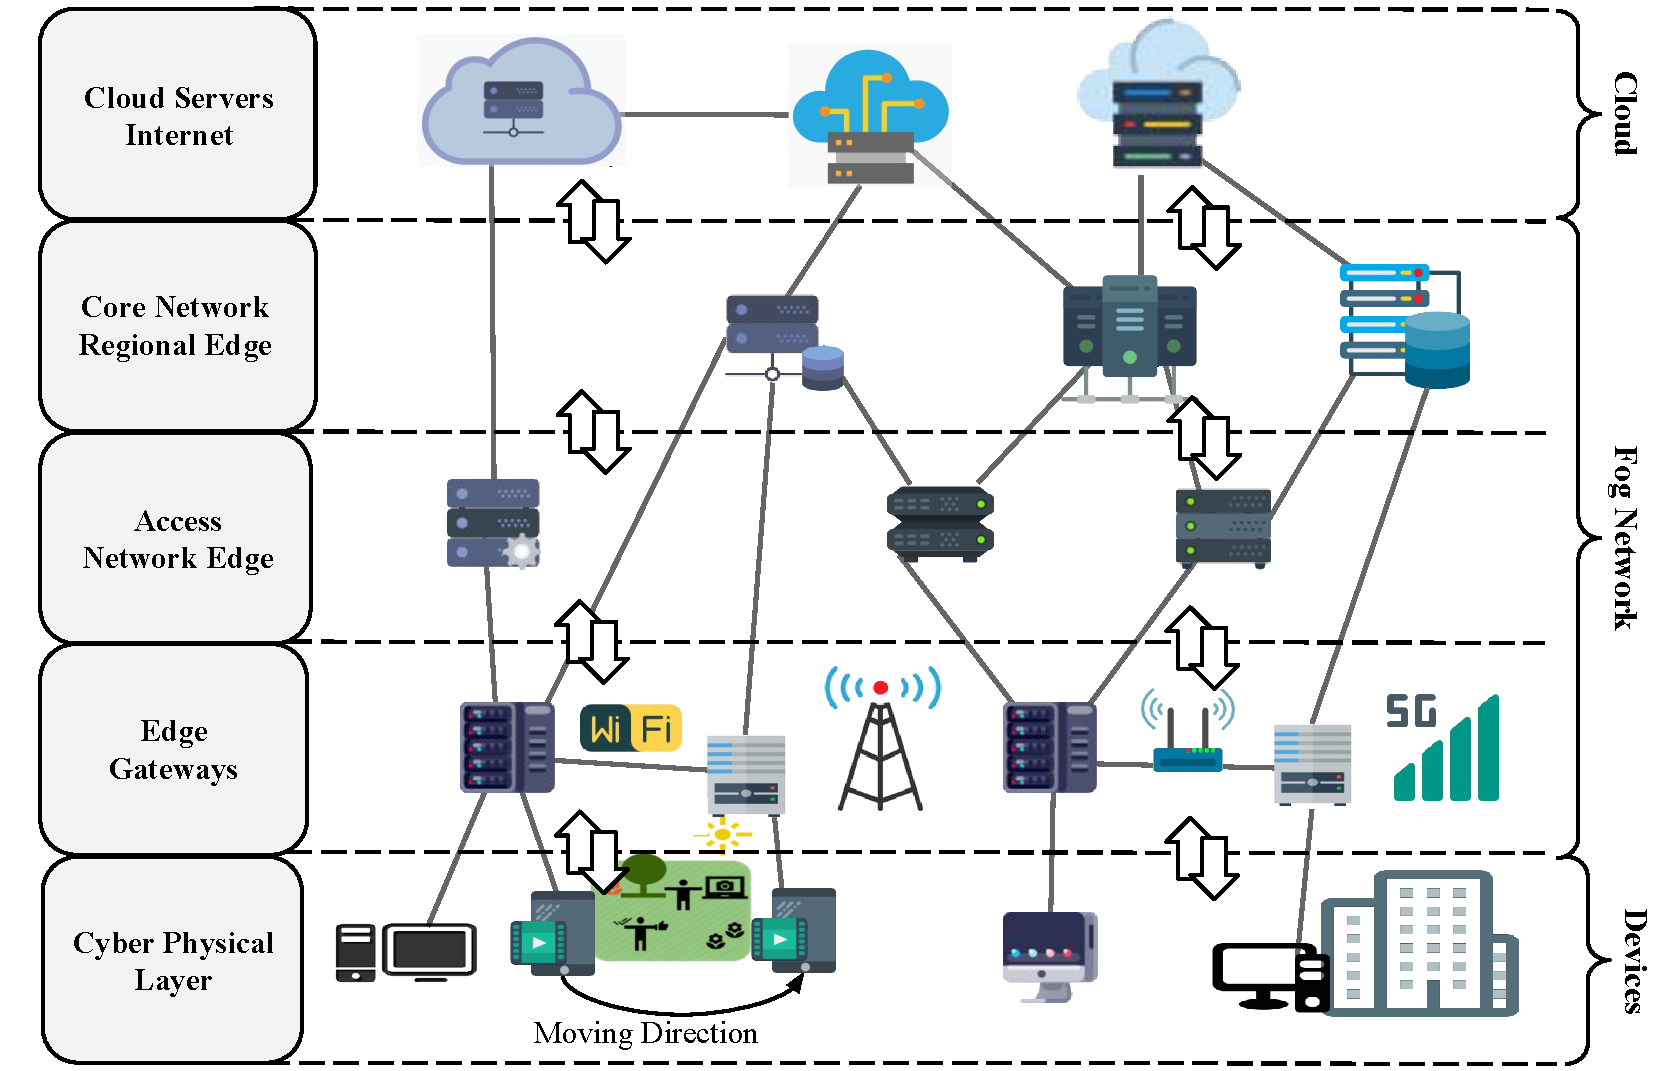
\includegraphics[scale=.5]{arch-multi-lvl}
  \caption{Main components of an multi-lvl environment.}
  \label{fig:ofswitch-components}
\end{figure}


%-----------------------------------------------------------------------------%
\subsection{HTTP Adaptative Streaming and MPEG-DASG standard}
\label{sec:has-dash}

In this proposal, we focus on video streaming applications based on MPEG-DASH (Dynamic
Adaptive Streaming over HTTP), a technology that dynamically
adapts to changing network conditions by requesting content in
chunks encoded at different bitrates, and which is used by major
streaming services like Netflix and YouTube.

Benefits
There are several key benefits in the adaption of this new standard. Due to the fact that several major media companies took part in its development, the new protocol will eliminate technical issues in delivery and compression. In essence, it aims to combine all of the technologies and standards into one, making streaming support seamless on all devices. In turn, it aims to reduce technical headaches and transcoding costs. Content publishers can generate a single set of files for encoding and streaming that should be compatible with as many devices as possible, from mobile to OTT, as well as to the desktop via plug-ins or HTML5. Consumers will not have to worry about whether their devices will be able to play the content they want to watch.

Characteristics
By parsing the MPD, the DASH client learns about the program timing, media-content availability, media types, resolutions, minimum and maximum bandwidths, and the existence of various encoded alternatives of multimedia components, accessibility features and required digital rights management (DRM), media-component locations on the network, and other content characteristics. 

Out of Scope
The MPEG-DASH specification only defines the MPD and the segment formats. The delivery of the MPD and the media encoding formats containing the segments, as well as the client behavior for fetching, adaptation heuristics, and playing content, are outside of MPEG-DASH’s scope.


\subsection{Aplicação CDN }
\section{Trabalhos Relacionados}
\label{ch:related-work}

Está seção busca mostrar os principais trabalhos relacionados a soluções em sistemas CDN e as tecnologias usadas para transmissão de conteúdo multimidia. 
Os projetos de arquitetura estão diretamente relacionados ao paradigma da computação em névoa para aplicativos de baixa latência. A disseminação de conteúdo concentra-se em reduzir a redundância da transmissão de dados nos nós de borda.
%The architecture designs directly related to fog computing paradigm for low latency applications. Content dissemination focus on reduce redundancy of data transmission on edge nodes.


% CDN-as-a-Service Provision Over a Telecom Operator’s Cloud
% Managing QoS Constraints in a P2P-Cloud Video on Demand System.
% OpenCache: A Software-defined Content Caching Platform.

\subsection{Arquiteturas Nuvem-Névoa}
\label{subsec:arch-cloud-fog}
% [ICC'15] Joint Content-Resource Allocation in Software Defined Virtual CDNs
% [CLCN'17] Optimal and Cost Efficient Algorithm for Virtual CDN Orchestration
% [CLCN'16] Scalable and Cost Efficient Algorithms for Virtual CDN Migration
% [ComNet'17] OPAC: An optimal placement algorithm for virtual CDN
Khedher~\textit{et al.}~\cite{khedherComNet2017, khedherLCN2017} destaca os princípios de Rede Definida por Software~(SDN) e Virtualização de Função de Rede~(NFV). A abordagem baseada em SDN/NFV permite funções específicas de virtualização em servidores remotos. Dessa forma, as migrações de serviços de conteudo multimidia podem ser virtualizadas em diferentes \textit{datacenters}. Os problemas de orquestramento e cache são abordados, seu trabalho desenvolve um algoritmo exato para decidir os locais ideais para alocação do serviço. O algoritmo proposto, incluindo o cache de conteúdo e o redirecionamento de solicitações, é introduzido com algumas restrições de QoE, de rede e sistema operacional. 
Desta forma, o gerenciamento do CDN é feito de maneira centralizada e utiliza o usuário final como alvo para fazer a comunicação Dispositivo para dispositivo, mas não explora a mobilidade. As solicitações de usuários finais serão redirecionadas para um local de nuvem de borda ideal, sem dispositivos de borda de nível com diferentes lantências. 

Llorca~\textit{et al.}~\cite{llorcaICCW2015} propõe uma rede de cache virtual implementada totalmente em software através de uma infraestrutura de rede em nuvem distribuída programável que pode ser consumida e otimizada elasticamente usando informações globais sobre condições de rede e requisitos de serviço chamados SDvCDN. Esta abordagem aborda os problemas de posicionamento (localização da instalação), roteamento~(rede de fluxo) e alocação de recursos~(design de rede).

% [SENSORS'18] Service Migration from Cloud to Multi-tier Fog Nodes for Multimedia Dissemination with QoE Support
Rosario~\textit{et al.}~\cite{rosarioSENSORS2018} apresenta uma arquitetura para servicos de migração ao vivo de VM da nuvem para multiniveis da fog. O cenario experimental a nuvem distribui o conteudo de video para os diferentes niveis da fog. A arquitetura é baseada no paradigma sdn para, distribuição de video com suporte a QoE. 
The work split the multi-tier fog in three tier in order to their cover, storage, upload and download capacity. Important aspects could be tailored to support generic content and IoT environments, besides work with both private and public clouds. A divisão da nuvem em multiniveis se dá pelas caracteristicas do  dispositivos conectado a nuvem, e não por qualquer interconexão entre esses aparelhos. The paper tem como focus prover tecnologias capazes de tornar este ambiente factivel, e melhorar o provisionamento de conteudo de servicos de stream de video.


% [ICC'17] Content Delivery Network Slicing: QoE and Cost Awareness
Retal~\textit{et al.}~\cite{retalICC2017} propõe uma plataforma de \textit{CDN as a Service (CDNaaS)} onde os usuário podem criar um \textit{slice} de CDN incluindo cache, transcodificador e \textit{streamers}, em ordem de gerenciar uma quantidade de videos para seus usuários. (Aborda CDN na nuvem)
% [JSAC'18] Optimal VNFs placement in CDN Slicing over Multi-Cloud Environment
Benkacem \textit{et al.} [JSAC'18] introduzir uma plataforma CDNaaS na qual um usuário pode criar uma fatia CDN definida como um conjunto de rede distribuída isolada de servidores de borda em domínios com várias nuvens, em que um servidor de borda hospeda um único VNF, como cache virtual, transcodificador virtual, streamer virtual e CDN- coordenador específico de fatia para o gerenciamento do ciclo de vida dos recursos de fatia e também para gerenciar vídeos e assinantes enviados. Essa plataforma foi projetada para ter o nível máximo de flexibilidade para reduzir uma fatia de CDN no topo de diferentes IaaS (Infraestrutura como Serviço) públicas e privadas, como Amazon AWS service, Microsoft Azure, Rackspace e nuvem gerenciada OpenStack. Além disso, a plataforma emprega mecanismos e algoritmos que criam fatias de CDN com reconhecimento de QoE com boa relação custo-benefício, envolvendo uma colocação ideal levando em conta o nível de QoE desejado. Portanto, o objetivo deste trabalho é encontrar um custo eficiente de CDN, respeitando, por um lado, os requisitos do proprietário da CDN em termos de QoE e, por outro lado, a infraestrutura em nuvem e seu custo.

% Adaptive Video Streaming with Network Coding Enabled Named Data Networking
Saltarin~\textit{et al.}~\cite{saltarinTrans2017} propõe uma arquitetura adaptável de streaming de vídeo pela NDN que usa codificação de rede para permitir o streaming ideal de vídeo com vários caminhos. Assim, o uso de vários caminhos para conectar os clientes às fontes aumenta a largura de banda vista pelos clientes, permitindo que os mecanismos de adaptação de qualidade do DASH convergam para melhores qualidades de vídeo do que com o uso de um único caminho de comunicação. Os clientes podem transmitir interesses por todas as suas interfaces de rede (por exemplo, LTE e Wi-Fi) para recuperar os pacotes de dados que compõem o conteúdo solicitado.
%Fig. 1. Devices retrieving Data packets over LTE and Wi-Fi: (a) multi-source unicast; (b) single-source multicast; (c) multi-source multicast (butterfly network).

%Shen \textit{et al.} [6] works with a set of cache proxy services to analyze the cache miss occurrences. This work implements a reactive approach where cache proxies download the chunks of multimedia content when requested.
Shen~\textit{et al.}~\cite{shenIWQoS19} trabalha com um conjunto de serviçosde cache, afim de analisar as ocorrências de falta de cache em servidores proxy. Este trabalho implementa uma abordagem reativa na qual os proxies de cache baixam os blocos de conteúdo multimídia apenas quando solicitados. Utilizando teoria da probabilidade para deduzir os valores mais adequados dos parâmetros críticos e fornecer orientações significativas para a seleção de valores para melhorar o QoE dos usuários.

\subsection{Serviços de Video Streaming Adaptativos}

% [1] QoE-fair Resource Allocation for DASH Video Delivery Systems
Cicco~\textit{et al.}~[1] aborda implementa uma estratégia de alocação de recursos justa. Para melhorar o QoE dos usuários, técnicas de engenharia de tráfego baseadas em slincing rede foram utilizadas. Ele mostra que a estrutura de otimização do Problema do Fluxo de Multi-Commodities~(MCFP) pode ser uma metodologia adequada para impor justiça em relação ao QoE dos usuários. Este artigo, em particular, primeiro mostra como converter nosso problema de alocação justa de recursos de QoE para um MCFP e, em seguida, propõe uma abordagem de agrupamento de tráfego para reduzir sensivelmente o número de fatias de rede e tornar o problema resultante tratável para distribuição de vídeo plataformas que atendem a um grande público. Essa abordagem de agrupamento atribui sessões de vídeo com base em uma métrica de similaridade proposta que depende da qualidade do vídeo.

% Want to Play DASH? A Game Theoretic Approach for Adaptive Streaming over HTTP
Bentaleb~\textit{et al.} desenvolve um Algoritmo de Teoria dos Jogos, um novo esquema de ABR orientado ao cliente que se esforça para selecionar a melhor taxa de bits baseada na moderna teoria dos jogos (GT) [13, 25]. Nossa solução permite uma colaboração eficiente entre diferentes entidades do DASH de maneira distribuída, sem sobrecarga explícita de comunicação, respeitando os requisitos de decisão dos players existentes do DASH e considerando o tráfego cruzado e as diferentes condições da rede. O GTA tem como objetivo alcançar um QoE de visualizador alto e estável.


% Client-Server Cooperative and Fair DASH Video Streaming
Altamimi \textit{et al.} 

%Google proposal
Zhang~\textit{et al.}~\cite{zhangINFOCOM17} concentra-se no lado do usuário, executando o nível médio de taxa de bits pelo algoritmo de adaptação à taxa de bits e a influência da variação do tamanho de segmentos para melhorar a QoE, enquanto que 

Poliakov~\textit{et al.}~\cite{poliakovPHD2018} implanta um streaming de vídeo DASH com várias fontes. O player do DASH-client pode baixar multiplos segmentos, ao mesmo tempo, através de diferentes conexões na nuvem. 

Archer~\textit{et al.}~\cite{archerGoogleJournal2019} propõe um algoritmo para lidar com as réplicas de cache para provisionamento de vídeo com largura de banda flash, o que é um gargalo crítico.

\subsubsection{Comparação entre trabalhos relacionados}
\label{subsec:applications}

As abordagens mencionadas em \autoref{subsec:arch-cloud-fog} podem diminuir a carga de tráfego 
e melhorar a QoE. No entanto, também existem armadilhas devido ao comportamento egoísta totalmente isolado (ou seja, essas soluções estão funcionando independentemente, sem coordenação) dos players do HAS.

Os trabalhos de streaming de video na seção 3.2 consegue este tipo de problema, surgem problemas nos cenários da Cidade Inteligente: mobilidade do usuário, esquemas de cache colaborativo em multiplos níveis, quantidade de usuários durante multidões de flash não são totalmente considerados. Neste projeto, pretendemos projetar um sistema de entrega de vídeo que considere esses problemas para melhorar a qualidade da experiência para uma variedade de necessidades de streaming de vídeo, incluindo requisitos de baixa latência.

%The aforementioned approaches could decrease the traffic load and improve QoE, but more
%issues arise in Smart City scenarios: user mobility, collaborative cache schemes over multi-edge,
%the amount of users during flash crowds, and interactive streaming requirements are not fully
%considered. In this project we aim to design a video delivery system that considers such issues
%to improve quality of experience for a range of video streaming needs, including low latency
%requirements.

Nesta parte, fornecemos uma comparação entre os trabalhos discutidos acima.
%de recursos entre vários esquemas de adaptação de taxa de bits de ponta em cada categoria. 
A Tabela~\ref{tab:comparison} resume essa comparação para cada artigo pesquisado em termos dos seguintes aspectos:

\begin{itemize}

\item Escalabilidade: O trabalho leva em consideração a escalabilidade apresentada em ambientes de cidades inteligentes? O número de usuários pode variar de acordo com o tempo e a mobilidade dos usuários.

\item \# de usuários: Quantos clientes estão incluídos nos experimentos? Único indica apenas um cliente, vários (poucos) indicam menos de 10 clientes e múltiplos (muitos) indicam mais de 10 clientes.

\item Heteregeneidade: O trabalho leva em consideração dispositivos com diferentes resoluções em seus experimentos?

\item Justiça: o trabalho leva em consideração a justiça entre vários clientes que compartilham a rede? Algumas soluções compartilham igualmente a largura de banda entre os clientes, indicados pelo BW, outros compartilham a largura de banda com base na qualidade perceptiva ou no QoE, indicados por QT e QoE, respectivamente.

\end{itemize}


\begin{table}[htb]
  \caption{Comparação com trabalhos relacionados.}
  \label{tab:comparison}
  \centering
  \scriptsize
  \begin{tabular}{p{2.8cm}p{2cm}p{2cm}p{2.2cm}p{2cm}p{2cm}}
    \toprule
    \textbf{Reference} &
    \textbf{Esquemas ABR} &
    \textbf{Escalabilidade} &
    \textbf{Mobilidade} &
    \textbf{\# de \newline usuários} &
    \textbf{Aproximação \newline Cooperativa} \\
    \midrule

    Hatem~\textit{et al.}~\cite{Ahmad2013a, Ahmad2013b} &
    Flow-based & Yes & \ac{DMM} gateways & No & No \\
    \addlinespace
    \addlinespace

    Llorca~\textit{et al.}~\cite{Banerjee2013} &
    Tunnel-based & Not discussed & Not discussed & Yes & Test bed \\
    \addlinespace
	\addlinespace
    Rosáio~\textit{et al.}~\cite{Basta2013a, Basta2014} &
    Tunnel-based & Yes & Not discussed & No & No \\
    \addlinespace
	\addlinespace
    Retal~\textit{et al.} \cite{Cho2014} &
    Tunnel-based & Not discussed & Aware & Yes & Test bed \\
    \addlinespace
	\addlinespace
    Benkacem~\textit{et al.} \cite{CostaRequena2014} &
    Flow-based & Yes & Aware & No & Test bed \\
    \addlinespace
	\addlinespace
    Saltarin~\textit{et al.} \cite{Ghazisaeedi2013} &
    Tunnel-based & Not discussed & Not discussed & Yes & Simulation \\
    \addlinespace
	\addlinespace
    Shen~\textit{et al.} \cite{Guerzoni2014} &
    Flow-based & Not discussed & Aware & Yes & No \\
    \addlinespace
	\addlinespace

%-------------------------------------------------------------------------------------

    Cicco~\textit{et al.} \cite{Gurusanthosh2013} &
    Tag-based & Yes & \ac{DMM} anchors & No & Analytical \\
    \addlinespace
	\addlinespace
	
    Bentaleb~\textit{et al.} \cite{Hampel2013} &
    Tunnel-based & Yes & Not discussed & Yes & No \\
    \addlinespace
	\addlinespace
	
    Altamimi~\textit{et al.} \cite{Jin2013a} &
    Tag-based & Yes & Aware & No & Test bed \\
    \addlinespace
	\addlinespace
	
    Zhang~\textit{et al.} \cite{Karimzadeh2014} &
    N/a & Yes & \ac{DMM} solutions & Not discussed & No \\
    \addlinespace
	\addlinespace
	
    Polliakov~\textit{et al.} \cite{Kempf2012a} &
    Tunnel-based & Not discussed & Not discussed & No & Test bed \\
    \addlinespace
	\addlinespace
	
    Archer~\textit{et al.} \cite{Kuklinski2014b} &
    N/a & Yes & Main focus & Not discussed & No \\
    \addlinespace
	\addlinespace
	
    \bottomrule
  \end{tabular}
\end{table}

\include{integration}
\clearpage
\section{Trabalho Desenvolvido}
\label{ch:developed}

Esta seção apresenta o trabalho realizado até o momento que auxilia o desenvolvimento 
deste projeto de pesquisa de doutorado. 

%This section presents the work carried out so far that is assisting the
%development of this doctoral research project. \autoref{sec:module} talks about
%some available software tools for performance evaluation and presents the new
%OpenFlow module for simulations. \autoref{sec:scenario} introduces the proposed
%\ac{SDN}-enabled \ac{LTE} simulation scenario, describing its design targets
%and the network topology. Finally, \autoref{sec:controller} describes the
%enhanced OpenFlow controller for the \ac{SDN}-enabled \ac{LTE} network.
% The work presented here is potential precursor of this doctoral research
% project.


%-----------------------------------------------------------------------------%
%\subsubsection{Comparison between the developed works}
%\label{subsec:applications}
%
%In this part, we provide a feature comparison between various state-of-the-art bitrate
%adaptation schemes in each category from the taxonomy in Figure 3.1. Table 3.1 summarizes
%this comparison for each surveyed paper in terms of the following aspects:

%-----------------------------------------------------------------------------%
\subsubsection{Formulação de Programação Linear Inteira~(ILP)}
\label{subsec:applications}

Nós podemos sobrepor uma rede fog-clod multinível para streaming de video e optimizar adaptativamente sua topologia para minimizar a latência de playback e melhorar o tempo de entrega de um video. A programação com reconhecimento de QoE resolve um programa inteiro linear.

Os vértices representam nós de rede e as arestas são os links de rede podendo ser com ou sem fio. Os links podem ser definidos por conexões físicas ou virtuais
Suponha que que existe $n$ usuários conectados na rede e $m$ servidores de streaming de videos, nós queremos encontrar um emparelhamento apropriado entre eles. Um \textit{matching} entre um usuários e um servidor é mostrado como um par $(i,j)$, e é associado com um benefio $a_{ij}$. O conjunto de usuários e servidores são denotados por $U$ e $V$, respectivamente.

\begin{itemize}
\item $\forall (i,j) \in S$, $i \in U$ e $j \in V$.

\item $\forall i \in U$, exite no maximo um par $(i,j) \in S$.

\item $\forall j \in V$, exite no maximo uma tripla $(i,j) \in S$.
\end{itemize}
 
%Com $V$ sendo o conjunto de todos os vertices, definimos uma atribuição $S$ como um conjunto de triplas $(i,j,k)$, considerando a arquitetura da Figura~[1]:

%\begin{itemize}
%\item $\forall (i,j,k) \in S$, $i \in D$ and $j \in U$ e $k \in V$.
%
%\item $\forall i \in D$, exite no maximo uma tripla $(i,j,k) \in S$.
%
%\item $\forall j \in U$, exite no maximo uma tripla $(i,j,k) \in S$.
%
%\item $\forall k \in V$, exite no maximo uma tripla $(i,j,k) \in S$ $\forall i \in M_{D}(i)$.
%\end{itemize}


A programação com reconhecimento de QoS resolve um programa inteiro linear que busca o valor da variável $x_{i,j} (\in (0, 1))$. $x_{i,j}$ é uma variável binária que assume os seguintes valores,

\vspace{0.5cm}
\begin{equation}\label{total_capacity_loss}
x_{i,j} =
\left\{\begin{matrix}
1, & \text{se um usuário \textit{i} é atribuído a um servidor \textit{j}} & \\ 
0, & \text{Caso contrário} & 
\end{matrix}\right.
\end{equation}
\vspace{0.5cm}

Em uma arquitetura multinível, os streamings de video tem um QoE diferente de acordo com os seus requisitos. Por exemplo, streaming em tempo real, como detecção on-line e streaming armazenado, são sensíveis a atrasos. Portanto, esses streamings devem ser processados o mais próximo possível do usuário final, de preferência em nós localizados no primeiro nível da névoa, enquanto que conteudos de video sob Demanda~(VoD) acenitam um atraso maior. Desta forma, vamos identificar cada stream de video requisitado pelos usuários finais por um identificador, a partir de agora simbolizado por "c".
Um nível de servidores, indicado por $S_{c}$, é um conjunto de nós que atende o QoE necessário para fornecer serviços de um stream de video específico, e nós definimos como um intervalo na forma de $S_{c} \in [a, b)$. onde $a_{c} < b_{c}$ e,

\vspace{0.5cm}
\begin{itemize}

\item  $c \in \{1,...,v\}$

\item  $a_{c} = \{a_{1},a_{2},...,a_{v}\}$

\item  $b_{c} = \{b_{1},b_{2},...,b_{v}\}$

\item  $a_{c},b_{c} \in N_{H}$

\end{itemize}
\vspace{0.5cm}

%Para simplificar esta formulação nós estamos considerando que os segmentos de video é requisitado a apenas um servidor fonte, e utiliza um interval de tempo discreto. Assim, $T = {1, ..., T max }$, onde $T_{max}$ é o tempo maximo que o video levaria para executar no nós mais rapido da fog. $T_{max}$ pode ser calculado como 
%
%\begin{equation}\label{minimize}
%T_{max} = \sum^{m}_{k} min(TI_{k | k \in N_{H}})
%\end{equation}

%Para melhor a latência da reprodução do video, nós devemos  minimizar a latencia de um nó para todas requisiçoes de segmentos do video. 

Para simplificar esta formulação nós estamos considerando que os segmentos de video é requisitado a apenas um servidor fonte, bem como o serviço de video streaming já está em execução em seus respectivos servidores. Colocando as limitações abaixo, An initial approach to the QoS-aware schedule is given by the following optimization problem:

\vspace{0.5cm}

%\begin{equation}\label{minimize}
%\text{minimize} \ \ \
%\sum^{\left | D \right |}_{i=1} 
%\sum_{\{j | (i,j,k) \in A\}}
%\sum_{\{k | (i,j,k) \in A\}}
%\frac{ c_{ijk} }{ m_{i}} \ast x_{ijk}
%\end{equation}

Maximizar

\begin{equation}\label{maximize}
\sum_{i \in U} 
\sum_{j \in S_{c}}
a_{ij} \ast x_{ij}
\end{equation}

Sujeito a

\begin{equation}\label{bound_1}
\sum_{\{j | (i,j,k) \in A\}}
\sum_{\{k | (i,j,k) \in A\}}
x_{ijk} = 1,  \forall i \in D
\end{equation}

\begin{equation}\label{bound_1}
\sum_{\{j | (i,j,k) \in A\}}
\sum_{\{k | (i,j,k) \in A\}}
x_{ijk} \leq 1,  \forall j \in U
\end{equation}

\begin{equation}\label{minimize}
\sum_{i \in U} 
\sum_{j \in S_{c}}
bw_{j} x_{ij}
\leq Bw_{j}
\end{equation}

\begin{equation}\label{minimize}
x_{ij}  \in  \{0, 1\}, \forall i \in U,j \in S_{c}
\end{equation}
\vspace{1.2cm}

Para melhorar o desempenho da rede, nós devemos atribuir todos os usuários aos respectivos streaming de video afim de maximizar o benefio total.
%A função objetivo minimiza o makepan do aplicativo fornecido por um planejamento.
%Para melhorar a latência da reprodução do video, nós devemos  minimizar a latencia de um nó para todas requisiçoes de segmentos do video. 
Logo, a função objetivo busca essa mximização. A primeira restrição requer que cada usuário seja atribuído a exatamente um servidor. A segunda restrição garante que cada usuário seja atribuído a no maximo um servidor. Afirma também que, se o número de usuários são maiores do que o número de lostas de download , alguns dos slots de upload permanecem sem atribuição. A terceira restrição garante que os slots de download em uma similaridade com a classe de download diferem de segmentos de video requisitados.

A restrição (6) evita a atribuição de mais um matching do que a capacidade de banda total disponível para cada servidor.

%-----------------------------------------------------------------------------%
\subsubsection{Formulação de Programação Linear Inteira~(ILP)}
\label{subsec:applications}


Para implementar os servidores DASH e os usuários que permitem o streaming de video adaptativo, modificamos o  Adaptive Multimedia Streaming com a base de código AMuSt~(AMuSt). 
A estrutura do AMuSt fornece um conjunto de aplicativos para produzir e consumir vídeo adaptável, com base no padrão DASH [2]. A funcionalidade DASH é fornecida pela biblioteca libdash [35], uma biblioteca de código aberto que fornece uma interface para o padrão DASH. Atualmente, libdash é o software de referência oficial do padrão DASH.
We consider that the end-users are interested in a video available in three different representations, Q = \{480p, 720p, 1080p\} with bitrates \{1750kbps, 3000kbps, 5800kbps\}, respectively, that are a subset of the ones used by Netflix in the past [11]. Each representation is divided into a set of 50 segments, each of a duration of 2 seconds.


\vspace{0.8cm}
\begin{figure*}[htpb]
	\centering
	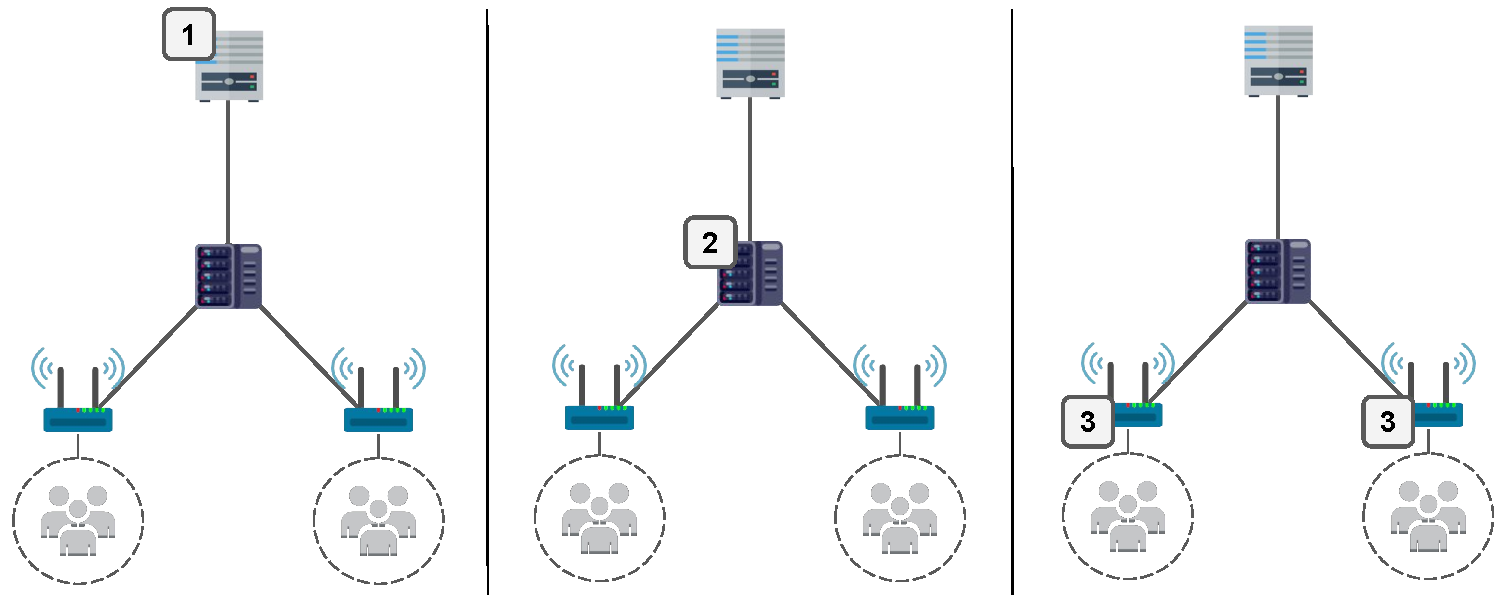
\includegraphics[width=0.75\textwidth]{img/exp-multi-lvl}
% 	\vspace{-1cm}
	\caption{DASH-based Adaptive Multimedia Delivery System for Cloud/Fog Nodes.}
	\label{fig:scenario-arch}
\end{figure*}


Avaliamos o impacto que uma arquitetura multinível de streaming de vídeo adaptativo em uma topologia com tres níveis com um único caminho, apresentada na Fig. 5. Os links possuem comprimento de possui um taxa de dados de 10 MBps e cada AP .


\vspace{0.8cm}
\begin{figure}[htb]
  \centering
    \subfloat[Taxa de bits medio.]
    {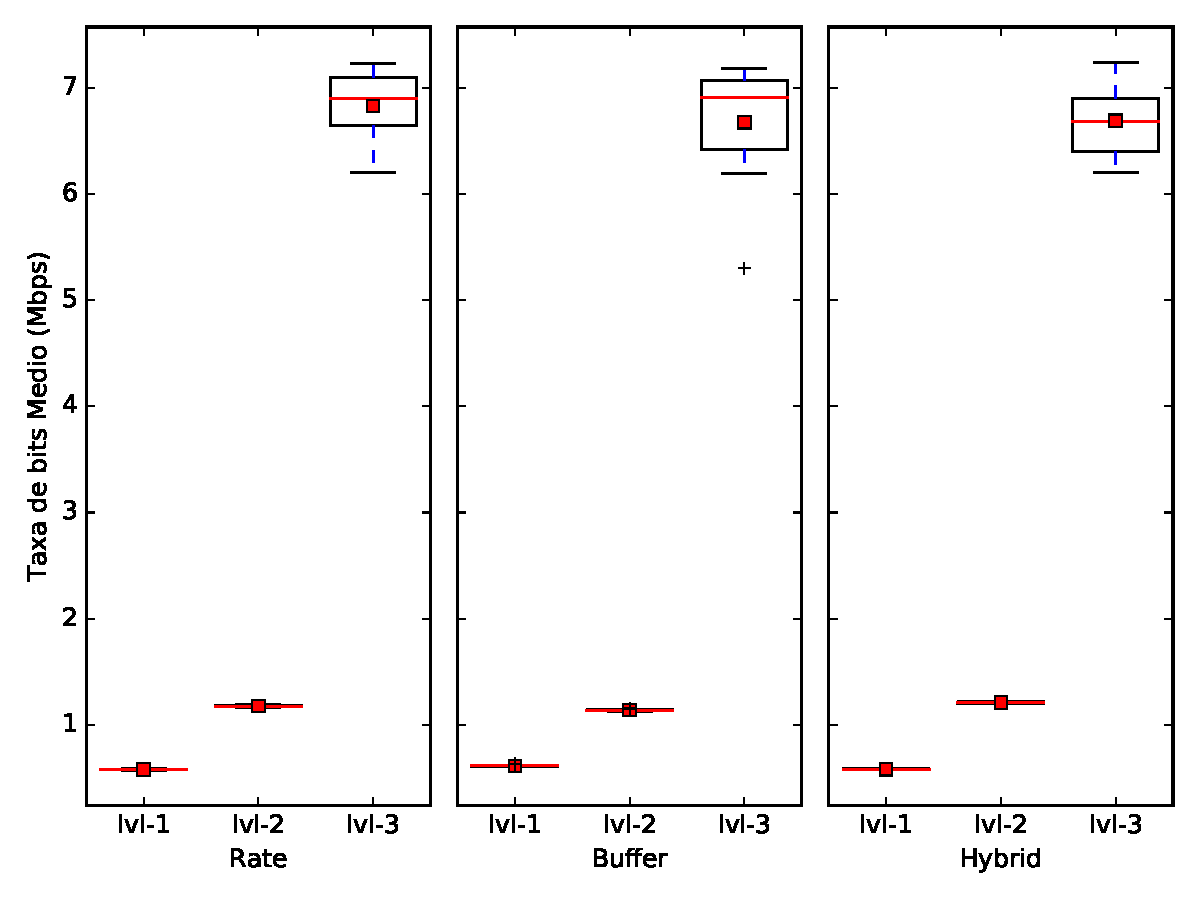
\includegraphics[width=.40\textwidth]{graphs/boxplot-avgBt}
    \label{fig:lte-handover}}
  \hfil \hspace{1cm}
    \subfloat[Tempo total de interrupções.]
    {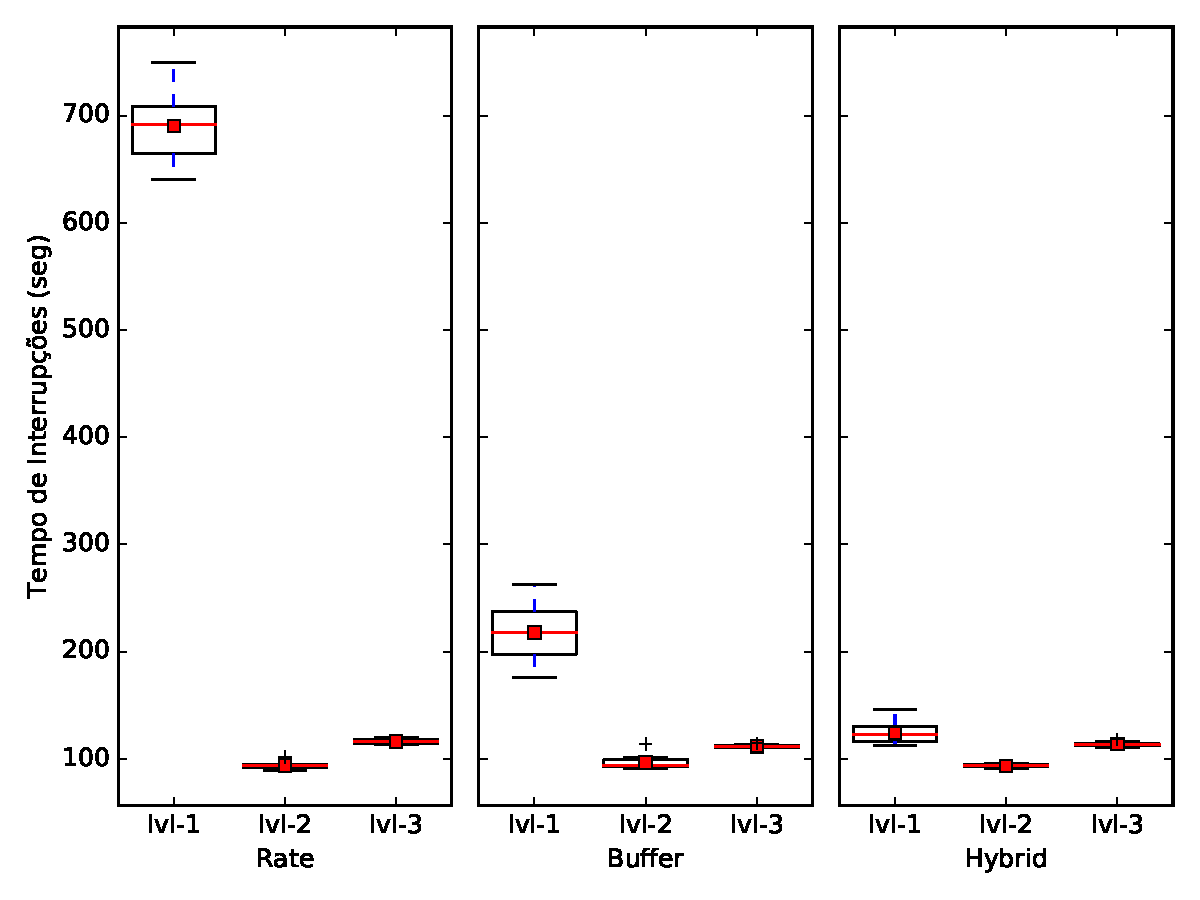
\includegraphics[width=.40\textwidth]{graphs/boxplot-avgStalls}
    \label{fig:dmm-proposal}}
  \caption{Resultados da taxa de bits media e tempo total de interrupções para uma rede com 10 em cada AP.}
  \label{fig:dmm}
\end{figure}

\begin{figure}[htb]
  \centering
    \subfloat[Taxa de bits medio.]
    {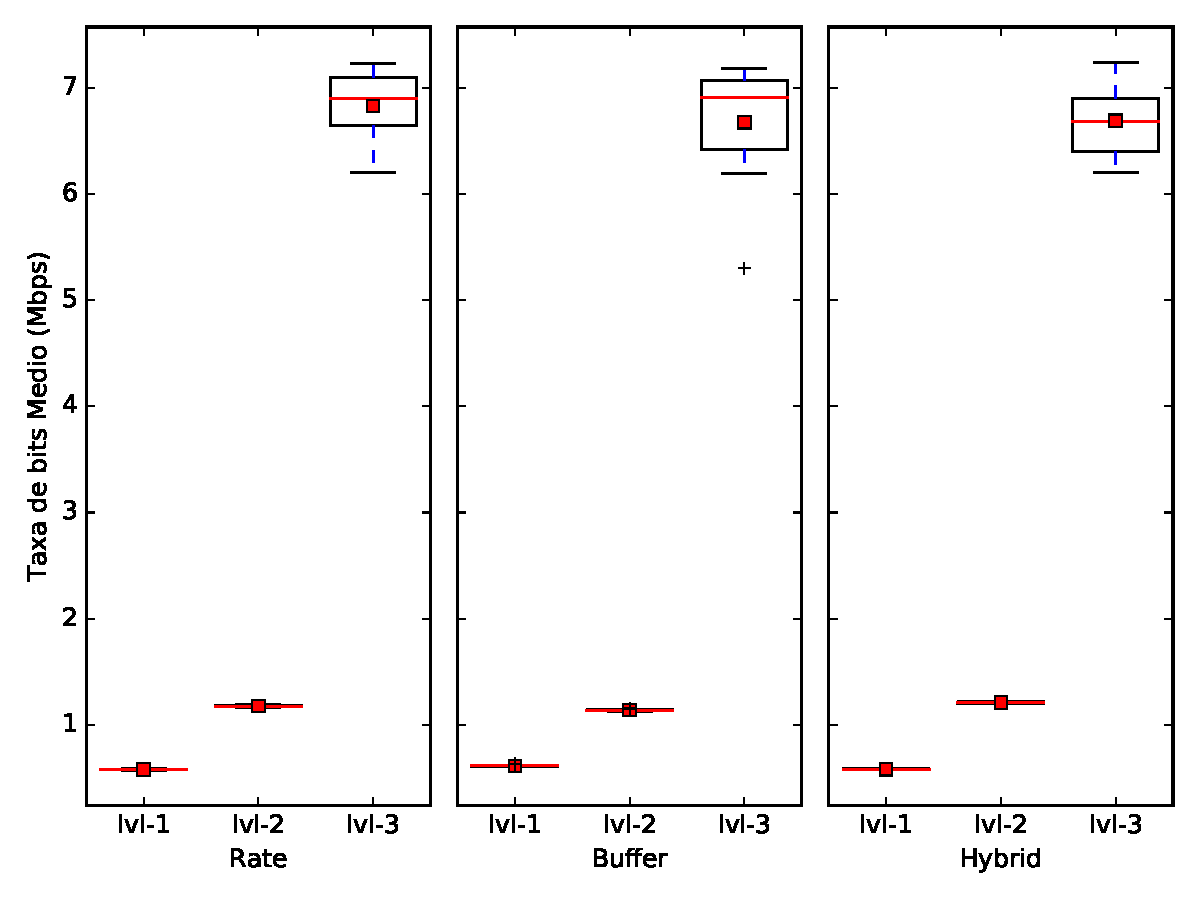
\includegraphics[width=.40\textwidth]{graphs/boxplot-avgBt}
    \label{fig:lte-handover}}
  \hfil \hspace{1cm}
    \subfloat[Tempo total de interrupções.]
    {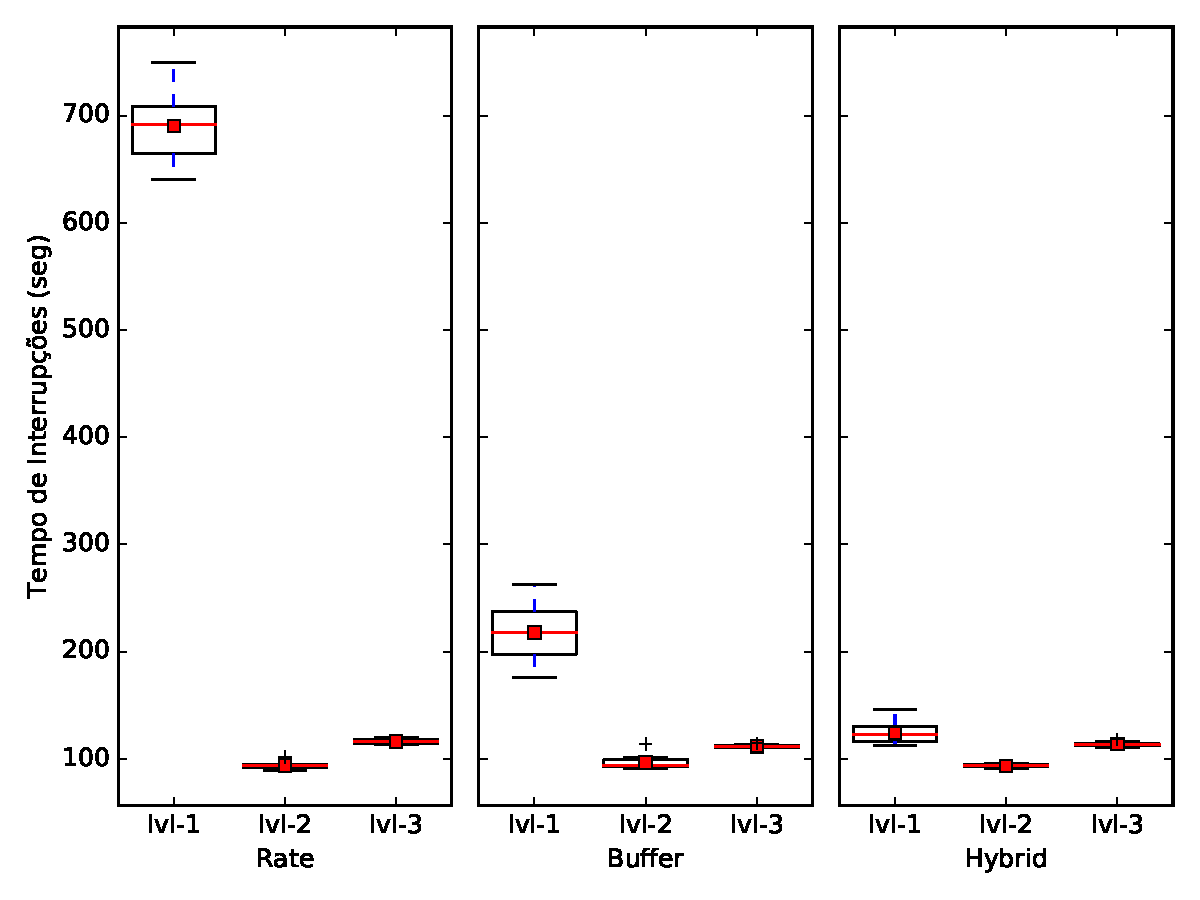
\includegraphics[width=.40\textwidth]{graphs/boxplot-avgStalls}
    \label{fig:dmm-proposal}}
  \caption{Resultados da taxa de bits media e tempo total de interrupções para uma rede com 10 em cada AP.}
  \label{fig:dmm}
\end{figure}
\clearpage
\section{Research topics to be investigated}
\label{ch:proposal}

This section presents some main ideas for the continuity of this doctoral
research project. \autoref{sec:topics} brings the research topics to be
addressed while \autoref{sec:timetable} shows the work plan and timetable.

%=============================================================================%
\subsection{Research topics}
\label{sec:topics}


Devido ao compartilhamento de ambientes de rede, a natureza do \textit{best-effort} da infraestrutura da Internet, e o comportamento egoísta totalmente isolado dos jogadores da HAS. é difícil para streams de vídeo satisfazer os três objetivos descritos abaixo. Desde de que existam multiplos clientes concorrentemente competindo entre eles um limitado comprimento de onda, as soluções existentes para clientes dirigido a HAS não trabalham vem e sofrem muitos problemas com perda de pacotes, flutação de comprimento de onda, oscilações na qualidado e troca de taxas de bits~(Instabiliddade do vídeo mostrada ba Figura~\TODO{Falta gerar gráfico}), QoE indesejavel e compartilhamento de recursos da rede, recursos da rede inutilizados ou sobrescritos do qual 'will adversely affect the viewer's QoE'. Alem disso, estes problemas tem sido confirmados em experimentos recentas. 

The research topics to be addressed are divided into three topics, which are
detailed in Sections~\ref{subsec:distributed} through \ref{subsec:handover}.
Each topic encompasses the motivation, goals, and objectives.

%-----------------------------------------------------------------------------%
\subsubsection{Scalable controller architecture}
\label{subsec:}

Este projeto tem como objetivo projetar uma entrega de vídeo baseada em DASH confiável e de alta qualidade para ser usada em ambientes de cidades inteligentes~\cite{gamaUCC2019, KreuzbergerWorkshop2016}. O esquema proposto aproveitará várias tecnologias relacionadas à rede, como Cloud, Fog e Edge Computing, além de posicionamento e encadeamento inteligente de serviços.% A Figura~\ref{fig:scenario-arch} descreve, no lado esquerdo, uma arquitetura de rede de várias camadas, composta por um conjunto heterogêneo de dispositivos e aplicativos que utilizam recursos de computação distribuídos por meio de uma tecnologia de comunicação de acesso múltiplo, como 5G e WiFi. Este projeto propõe estender o streaming de vídeo DASH para suportar conectividade simultânea de caminhos múltiplos~\cite{poliakovPHD2018, Velasquez2018}.

%O lado direito da Figura~\ref{fig:scenario-arch} descreve parte dos parâmetros que devem ser avaliados para definir quais serviços de vídeo precisam ser implantados, juntamente com a camada mais adequada para implantar cada um deles. Observe que os parâmetros na camada mais inferior para feedback diferem dos de outras camadas. Inicialmente, os parâmetros avaliados considerados incluem o perfil do usuário, a carga da célula local, a qualidade do link, a complexidade do movimento dos vídeos e também detalhes inteligentes da cidade, como a localização e a rota rastreada no caso de usuários com mobilidade. Alguns dos nós podem ser estacionários, mas outros podem variar de padrões de baixa a alta mobilidade, que podem ser levados em consideração para melhorar a qualidade da entrega de vídeo.

\vspace{0.8cm}
\begin{figure*}[htpb]
	\centering
	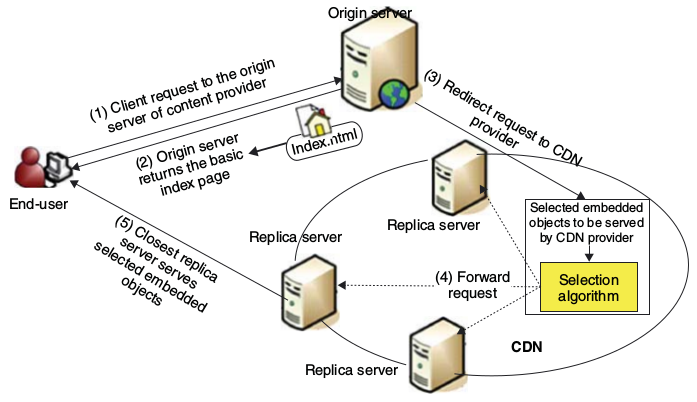
\includegraphics[width=0.7\textwidth]{img/fig-intro.png}
% 	\vspace{-1cm}
	\caption{DASH-based Adaptive Multimedia Delivery System for Cloud/Fog Nodes.}
	\label{fig:scenario-arch}
\end{figure*}

Dada a arquitetura do modelo de serviço e ambiente de nuvem/borda de várias camadas mencionada, este trabalho tem como objetivo abordar algumas das seguintes questões de pesquisa:~\textit{i)} Como determinar as melhores camadas para alocação de serviços de vídeo?~\textit{ii)} Como os pedaços de vídeo não solicitados devem ser distribuídos na hierarquia de borda/nuvem, considerando as informações de localização do usuário e estimativas sobre a localização futura do usuário em tempo real?~\textit{iii)} Como facilitar o streaming de vídeo através de várias fontes simultaneamente?~\textit{iv)} Como os algoritmos de adaptação à taxa de bits podem ser afetados pelo tamanho do pedaço de vídeo em uma arquitetura de várias camadas?

\subsection{Multimedia Delivery System Schemes}
% Selection Algorithms

\subsection{Game Theory Based Adaptative Bit Rate Scheme}

% This project aims to design a reliable and high-quality DASH-based video delivery to be used in Smart City Environments~\cite{gamaUCC2019, KreuzbergerWorkshop2016}. The proposed scheme will take advantage of several network-related technologies such as Cloud, Fog, and Edge Computing, as well as intelligent service placement and chaining. Figure~\ref{fig:scenario-arch} depicts, on its left-hand side, a multi-tier network architecture, which is composed of a heterogeneous set of devices and applications using distributed computing resources through a multi-access communication technology, such as 5G and WiFi. This project proposes to extend DASH video streaming to support simultaneous multipath connectivity~\cite{poliakovPHD2018, Velasquez2018}.

% The right-hand side of Figure~\ref{fig:scenario-arch} describes part of the parameters that should be assessed to define which video services are needed to be deployed along with the most suitable tier to deploy each of them. Note that the parameters in the bottommost tier for feedback differ from those of other tiers. Initially, the assessed parameters considered include the user's profile, the load of the local cell, the link quality, the motion complexity of the videos, and also smart city details such as the location and the traced route in case of users with mobility. Some of the nodes can be stationary, but others can range from low to high mobility patterns, which can be taken into account to improve quality of video delivery.

% \vspace{0.8cm}
% \begin{figure*}[htpb]
% 	\centering
% 	\includegraphics[width=1.0\textwidth]{images/scenario_incomplete}
% % 	\vspace{-1cm}
% 	\caption{DASH-based Adaptive Multimedia Delivery System in an Smart City Environment.}
% 	\label{fig:scenario-arch}
% \end{figure*}

% Given the aforementioned multi-tier edge/cloud environment and service model architecture, this work aims to tackle some of the following research questions:~\textit{i)} How to determine the best tiers for video services placement?~\textit{ii)} How unsolicited video chunks should be distributed in the edge/cloud hierarchy considering user location information and estimates on future user location in real time? ~\textit{iii)} How to facilitate video streaming through multiple sources concurrently?~\textit{iv)} How bitrate adaptation algorithms can be impacted by video chunk size in a multi-tiered architecture?


% Neste trabalho, queremos construir um sistema CDN na fog com o uso de cache e sobreposição de rede para para streaming de video ao vivo, e otimizar sua topologia de forma adaptativa para minimizar a latência de reprodução média e melhorar a entrega do fluxo de forma oportuna. A latência de reprodução é a diferença entre o tempo de reprodução (ponto de reprodução) na origem de mídia e em um nó.

% \vspace{1cm}
% \noindent
% \textbf{Modelagem de propriedades de balanceamento de carga e desempenho de cache em sistemas de Névoa-Nuvem multicamadas.}

%-----------------------------------------------------------------------------%
\subsection{Medidas objetivas}


%-----------------------------------------------------------------------------%
\subsubsection{Scalable controller architecture}
\label{subsec:distributed}

\emph{The goal of this research topic is} to improve the current controller
model toward a scalable architecture. \autoref{fig:distributed-controller}
shows a possible distributed \ac{EPC} controller architecture, where the
\acp{eNB} are enhanced with a local controller and switch that are used for
traffic classification purposes at the network edge. A centralized topology
controller can independently handle topology-related questions (like traffic
routing) in the backhaul network. Finally, a specialized \ac{QoS} controller
would be in charge of admission control and \ac{QoS} management, communicating
with edge and topology controller. Theses controllers can be assisted by
applications, like network mapper and routing and a more sophisticated
admission control software. 
\emph{The objectives for this research topic are:}
\begin{itemize}
  \item Determine the controller functionalities that can be performed
  independently of each other, to effectively proposed a distributed controller
  architecture;

  \item Model the inter-controller communication for the distributed controller
  architecture, reducing the amount of information exchanged between
  controllers;

  \item Evaluate possible standardized east/westbound interfaces for controller
  interaction;

  \item Implement and evaluate the proposed architecture in the \ac{ns-3}
  simulator, performing scalability tests with large numbers of \acp{eNB} and
  \acp{UE} in the network.
\end{itemize}

%-----------------------------------------------------------------------------%
\subsubsection{Traffic offloading in \acsp{HetNet}}
\label{subsec:heterogeneous}

As the wireless link efficiency is approaching its fundamental limits, further
improvements in cellular system spectral efficiency are only possible by
increasing the node deployment density. As observed by \citet{Damnjanovic2011},
challenges associated with the deployment of traditional macro base stations
can be overcome by the utilization of base stations with lower transmit power.
A network that consists of a mix of macro cells and low-power nodes, where some
may be configured with restricted access and some may lack wired backhaul, is
referred to as a \acf{HetNet}. \autoref{fig:hetnet} exemplifies a \ac{HetNet}
with a macro cell, some metro and picocells used for relay, some network
operator deployed low-costs indoor and outdoor small cells, and user deployed
very low costs for indoor environment.

\begin{figure}[htb]
  \centering
  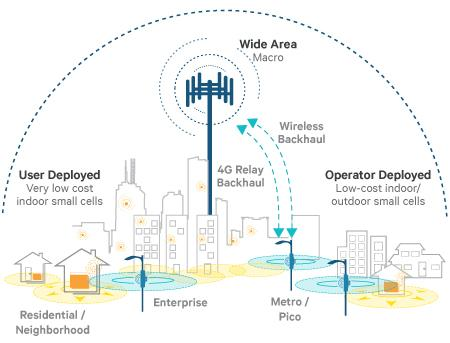
\includegraphics[scale=0.55]{hetnet}
  \caption{A \acs{HetNet} example scenario~\cite{Qualcomm2014}.}
  \label{fig:hetnet}
\end{figure}

The future 5G architecture must provide a communication environment able to
overcome the infrastructure shortcomings of current networks. Networks will
become much denser with many more cells with decreasing size as well as direct
device-to-device communication. Small cells improve capacity and cellular
coverage with lower cost compared to macrocells, and they are expected to carry
the majority of traffic. \citet{Pierucci2015} says that while bringing the base
station closer to the user, it is possible to promote lower power use and more
energy efficient communications. In the opinion of \citet{Einsiedler2015}, the
vision is to provide functional convergence of network control to handle 5G,
4G, older access technologies, and Wi-Fi; enabling a flexible and efficient
support and deliver all types of applications.

As claimed by \citet{Tomici2015}, network operators have shown more interest in
deploying integrated small cell and Wi-Fi accessing networks to accommodate the
increasing demand for bandwidth caused by widespread wireless data usage.
However, the 3GPP interworking architecture forces the inter-system handover to
happen solely at the \ac{P-GW}, which may cause unnecessary burdens on the
mobile core network, especially with the expected large number of small cell
and Wi-Fi accessing network deployment.

Within an \ac{SDN} architecture, the user data plane can be distributed to
allow local offloading of user data traffic, regulated by the (partially)
logically centralized network controller. An example of traffic offloading
solution is the one proposed by \citet{Ghazisaeedi2013}, where a switching
system is used to redirect \ac{HTTP} traffic from \ac{S-GW} to the Internet.
This technique can decrease the traffic load over the mobile core network. In
\citet{Tomici2015}, the authors suggest three new \ac{LTE}-\ac{WLAN}
integration architectures for inter-system handover, which are based on having
a local integration point. For each of these integrated architectures, the
authors propose a network-initiated inter-system handover mechanism between the
\ac{eNB} and \ac{WLAN} \ac{AP}. The handover mechanisms are efficient due to
limited interaction with the \ac{P-GW} in the core network.

\emph{The goal of this research topic is} to design an algorithm responsible
for offloading \ac{LTE} traffic over available Wi-Fi networks. Assuming that
many Wi-Fi hotspots are deployed by the mobile operators in public urban areas,
the algorithm focus is to trigger offloading decisions based on the current
traffic load in the backhaul and core networks.
\emph{The objectives for this research topic are:}
\begin{itemize}
  \item Compare current approaches for traffic offloading in mobile networks,
  identifying the benefits and drawbacks of each solution;

  \item Propose an improved offloading decision solution for \ac{EPC}, using
  Wi-Fi as enabler technology;

  \item Implement and evaluate the proposed solutions in the \ac{ns-3}
  simulator, performing tests on scenarios with different access networks.
\end{itemize}

%-----------------------------------------------------------------------------%
\subsubsection{Distributed mobility management}
\label{subsec:handover}

Mobility management refers to a set of mechanisms to keep ongoing sessions
continuity while a mobile user changes its mobility anchor point in the
network. In the \ac{LTE} architecture, mobility management solutions rely on
centralized mobility anchor entities (\ac{S-GW} and \ac{P-GW}), which are in
charge of both mobility-related control plane and user data forwarding.
According to \citet{Valtulina2014}, this centralized approach makes mobility
management prone to several performance limitations such as suboptimal
routing, low scalability, potential single point of failure and the lack of
granularity for the mobility management service.

Nowadays, \acf{DMM} is considered as a promising solution to solve these above
challenges. Several proposals tried to redesign mobile network architecture by
leveraging \ac{SDN} and OpenFlow with the support of \ac{DMM}.
\citet{Karimzadeh2014} discuss the \ac{DMM} in \ac{LTE} systems composed of
virtual gateways running on the cloud. \citet{Kuklinski2014b} discuss the
evolution of mobility management mechanisms in mobile networks and how \ac{SDN}
can be applied to efficiently handle mobility in the context of future 5G
networks. In the CROWD architecture~\cite{Ahmad2013a}, a \ac{DMM} gateway
replaces current anchor points, and mobility management functions are executed
by control applications. \citet{Gurusanthosh2013} propose the \acf{SDMA} in
\ac{LTE} backhaul access networks, including detailed handover procedure with
dynamic anchor element choice, which is based on \ac{UE} location and path
changes during handover. \citet{Mahmoodi2014} introduce a distributed \ac{SDN}
control plane with mobility management as an example where the controller
becomes responsible for handover procedures, reducing the power consumption of
the \ac{UE} and the signaling message overhead between entities at the backhaul
side.

Besides, mobility management may no longer be exclusively triggered by radio
quality, but also by network management decisions~\cite{Rost2014}. Several
redesigned handover procedures are proposed by \citet{Zhang2015b} for 5G ultra
dense networks. They take advantage of control and user-plane separation,
taking into consideration of mobility, stability, energy efficiency and
realizability.

Particularly, handover performance can severely impact the \ac{QoS} in
\acp{HetNet}. The increasing number of small nodes bring cells closer and there
is no more obvious boundary between them, enhancing the capacity per area by
the space division multiplexing. \citet{Sun2015} propose intelligent schemes
to handle the dynamic environment of \acp{HetNet}. The authors identify some
key problems in 5G \acp{HetNet} as traffic control, load balancing, density
prediction, and resource allocation. Then, they develop a number of smart
schemes to overcome these challenges.

\emph{The goal of this research topic is} to distribute the mobility management
computation intensive task among the \ac{MME} and a number of controllers nodes
in the network, avoiding a centralized operation. The handover processing can
also be assisted by a sophisticated software application. With this approach,
it is possible to reduce signaling overhead over backhaul and core network and
speed up handover procedures. The development of such distributed solution will
be guided by group handover in heterogeneous environments, when a group of
users may change the access networks simultaneously or within short
time~\cite{Chowdhury2012}.

Another opportunity is to explore \ac{SDN} flexibility and move the anchor
point to the OpenFlow backhaul network, considering that when a \ac{UE} is
handed over to a new access point, in most cases a large part of the path that
the traffic takes in the backhaul network would be the same before and after
the handover. \autoref{fig:lte-handover} shows how \ac{GTP} tunnels are handled
during a normal handover procedure in \ac{LTE} networks, and
\autoref{fig:dmm-proposal} exemplifies how the proposed distributed mobility
management solution can handle the \ac{GTP} tunnels, following some ideas from
the \ac{SDMA}. Nonetheless, while \ac{SDMA} demands changes in the standard
procedures with no backward compatibility, the proposed solution must be
designed to offer interoperability with existing networks.

\begin{figure}[htb]
  \centering
    \subfloat[Centralized anchor.]
    {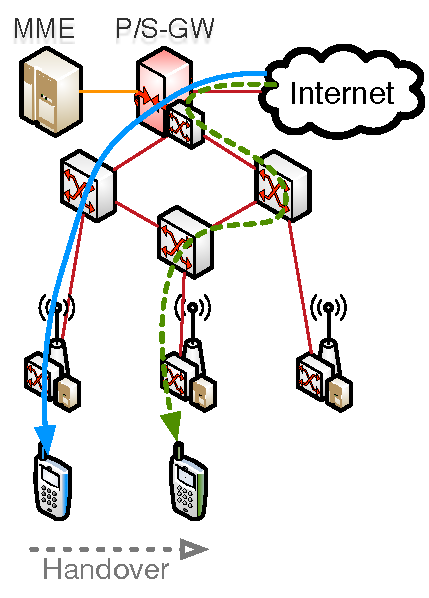
\includegraphics[width=.25\textwidth]{lte-handover}
    \label{fig:lte-handover}}
  \hfil \hspace{1cm}
    \subfloat[Distributed anchor.]
    {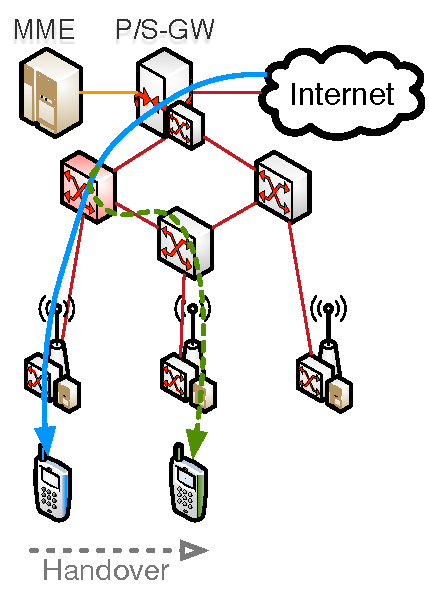
\includegraphics[width=.25\textwidth]{dmm-proposal}
    \label{fig:dmm-proposal}}
  \caption{\acs{SDN}-enabled \acs{LTE} network topology.}
  \label{fig:dmm}
\end{figure}

\emph{The objectives for this research topic are:}
\begin{itemize}
  \item Detailed study of \ac{LTE} handover procedures to propose a suitable
  distribution among \ac{MME} and available OpenFlow controllers, considering
  the interoperability with \ac{3GPP} standards;

  \item Examine available solutions for load balancing in mobile networks,
  which can be used to trigger handover procedures in the distributed
  architecture;

  \item Analyze existing solutions for vertical handover in \acp{HetNet},
  taking care of handovers between overlapping macro and small cells;

  \item Assess approaches for rerouting tunnels in OpenFlow backhaul network,
  looking for an optimal anchor element;

  \item Implement and evaluate the proposed \ac{DMM} in the \ac{ns-3}
  simulator, performing handover tests with groups of \acp{UE} between
  \acp{eNB}.
\end{itemize}


%=============================================================================%
\subsection{Work plan and timetable}
\label{sec:timetable}

\autoref{tab:timetable} presents the timetable for this doctoral research
project. The activities referenced in the timetable are listed below and
comprises both the developed work introduced in \autoref{ch:developed} and the
topics to be investigated from \autoref{sec:topics}. The activities that are
already developed are identified by the symbol~\,\m. Meanwhile, the symbol
\,\x\, identifies the expected time for carrying out the planned activities.

\begin{enumerate}
	\itemsep0pt
  \item Detailed study on \ac{SDN} and \ac{LTE} integration;
  \item Evaluation of available software tools for performance analysis;
  \item Development of the OpenFlow 1.3 module for \ac{ns-3};
  \item Proposal of the \ac{SDN}-enabled \ac{LTE} network;
  \item OpenFlow \ac{EPC} controller for traffic routing and bearer admission
        control;
  \item \ac{LTE} \ac{QoS} realization with OpenFlow protocol;
  \item Doctoral qualifying exam writing and defense;
  \item Scalable controller architecture proposal;
  \item Traffic offloading in heterogeneous networks;
  \item Distributed mobility management solutions;
  \item Thesis writing and defense.
\end{enumerate}

\begin{table}[htb]
  \renewcommand{\arraystretch}{1.4}
  \caption{The timetable for this doctoral research project.}
  \label{tab:timetable}
  \tiny
  \centering
  \begin{tabular}{c|c|cccc|cccc|cccccc|c}
    \toprule
    & {\bf 2013}
    & \multicolumn{4}{c|}{{\bf 2014}}
    & \multicolumn{4}{c|}{{\bf 2015}}
    & \multicolumn{6}{c|}{{\bf 2016}}
    & {\bf 2017} \\

    & {\it Oct} & {\it Jan} & {\it Apr} & {\it Jul} & {\it Oct} & {\it Jan} &
    {\it Apr} & {\it Jul} & {\it Oct} & {\it Jan} & {\it Mar} & {\it May} &
    {\it Jul} & {\it Sep} & {\it Nov} & {\it Jan} \\

    & {\it Dec} & {\it Mar} & {\it Jun} & {\it Sep} & {\it Dec} & {\it Mar} &
    {\it Jun} & {\it Sep} & {\it Dec} & {\it Feb} & {\it Apr} & {\it Jun} &
    {\it Aug} & {\it Oct} & {\it Dec} & {\it Feb} \\
    \hline % \midrule
    \arrayrulecolor{lightgray}

    %        |2013|       2014        |       2015        |            2016             |2017
    %        | 08 | 01   04   07   10 | 01   04   07   10 | 01   03   05   07   09   11 | 01
    %        | 12 | 03   06   09   12 | 03   06   09   12 | 02   04   06   08   10   12 | 02
    {\bf 01} & \m & \m &    &    &    &    &    &    &    &    &    &    &    &    &    &    \\ \hline
    {\bf 02} &    & \m &    &    &    &    &    &    &    &    &    &    &    &    &    &    \\ \hline
    {\bf 03} &    & \m & \m & \m & \m &    &    &    &    &    &    &    &    &    &    &    \\ \hline
    {\bf 04} &    &    &    & \m & \m & \m &    &    &    &    &    &    &    &    &    &    \\ \hline
    {\bf 05} &    &    &    &    &    & \m & \m & \m &    &    &    &    &    &    &    &    \\ \hline
    {\bf 06} &    &    &    &    &    &    &    & \m & \m &    &    &    &    &    &    &    \\ \hline
    {\bf 07} &    &    &    &    &    &    &    &    & \x & \x &    &    &    &    &    &    \\ \hline
    {\bf 08} &    &    &    &    &    &    &    &    & \x & \x & \x &    &    &    &    &    \\ \hline
    {\bf 09} &    &    &    &    &    &    &    &    &    & \x & \x & \x & \x & \x &    &    \\ \hline
    {\bf 10} &    &    &    &    &    &    &    &    &    &    &    & \x & \x & \x & \x &    \\ \hline
    {\bf 11} &    &    &    &    &    &    &    &    &    &    &    &    &    & \x & \x & \x \\

    \arrayrulecolor{black}
    \bottomrule
  \end{tabular}
\end{table}



%=============================================================================%
\section{Motivação}

%Este projeto propõe o uso da hierarquia de borda/nuvem para projetar um streaming de vídeo DASH cooperativo nas Smart Cities, implantando o serviço de cache para oferecer melhor qualidade de experiência~(QoE) para os usuários finais.
%At the same time, video streaming services represent the majority of the internet traffic, and according to Cisco forecasts\footnote{Cisco Visual Networking Index: Global Mobile Data Traffic Forecast Update. Link:~\url{http://shorturl.at/hjAZ1}. Accessed: July 29, 2019.}, in 2021 70\% of all internet traffic will be dominated by video streaming. This includes current video services as well as innovative services such as cloud gaming and future consoles (e.g. Google Stadia), whereas for mobile devices this estimate represents 78\% of all mobile data traffic. To accommodate video traffic, a good cloud-level architecture partially solves some issues related to the live stream and Video on Demand~(VoD) services. However, a centralized cloud service introduces some issues such as higher latency and core network congestion. Therefore, to improve video services, it is of paramount importance to properly distribute video streams according to their requirements: a cloud gaming infrastructure is an interactive service that needs reduced delays (a few milliseconds), while a non-interactive VoD delivery can tolerate higher delays without impairing quality of experience. A proper management and orchestration of video delivery over the Internet is core to the smooth co-existence of heterogeneous video services. This project proposes the use of edge/cloud hierarchy to design a cooperative DASH video streaming in Smart Cities, deploying cache service to offer improved Quality of Experience~(QoE) for end-users.

%*********** about IOT ******************


%***********Objectives of the proposal***********
1. How to deliver high quality streaming using in-Network coding and caching?
2. How to enable the multipath and multicast capabilities for HAS in future networks like ICN?
3. What is the impact of these networks on HAS decisions?
4. What is the benefits that edge computing can add in HAS over the future networks?
5. What is the deployment cost?


\section{Problem Statement}

The most of the exiting HAS delivery solutions, and their ABR schemes have four major shortcomings which are summarized as follows:

1. Multi-player problem.

2. Bandwidth fluctuation problem.

3. Quality fairness and heterogeneous system problem.

4. Trade-off between QoE metrics and ABR objectives problem.

\clearpage
\section{Final remarks}
\label{ch:remarks}

This research proposal is intended to explore the potentials of \acl{SDMN}. 
% ----------------------------------------------------------------------------
% How the SDN paradigm can be actually used to expand existing networks, moving
% away the vendor dependence but sustaining the performance achieved by
% dedicated hardware? 
% ----------------------------------------------------------------------------
Through a comprehensive literature review, it is possible to observe how the
existing solutions can improve mobile networks toward \ac{SDMN}. Different
approaches are used to simplify the equipment and increase flexibility due to
\ac{SDN} centralized control.
% ----------------------------------------------------------------------------
% How the proposed solutions are evaluated and what is the effective adoption
% of these solutions? 
% ----------------------------------------------------------------------------
There are many proposals in the area, but the performance evaluation processes
for new solutions is not uniform. Some solutions have no performance validation
while other works evaluate their proposals using small software test bed. To
overcome this need, a new OpenFlow module was developed, allowing \ac{ns-3}
simulations in this area. In addition, a new simulation scenario has been
proposed, and the current centralized controller architecture is to be
distributed among local agents in the direction of a scalable solution.
% ----------------------------------------------------------------------------
% How to manage upcoming heterogeneous 5G networks, considering different radio
% technologies and the explosion of connections? 
% How to effectively simplify mobility management in current architectures,
% exploiting the SDN centralized network view?
% ----------------------------------------------------------------------------
Taking into account that future 5G networks will become much denser with many
more cells, another item of interest in this research is how to perform user
handover and traffic offloading between different cells, and even between
different technologies. To this end, it is proposed a distributed mechanism for
dealing with mobility management decisions.



\setlength{\bibsep}{7.5pt}
\singlespacing
\footnotesize{
  \bibliographystyle{apalike}
  \bibliography{references}
}

\end{document}

\grid
\grid
\grid
\grid
